% !TEX root = ../Thesis.tex
\chapter{Implementation}

In this section, we will introduce how we implement a word-gesture keyboard using Unity, a Python script and a simpplified version of the word detecting algorithm used in $\text{SHARK}^2$.

\section{Word Graph Generator}
As previously discussed in section \ref{SHARK2}, to make $\text{SHARK}^2$ work, the perfect graphs for all words in a lexicon must be precomputed. Therefore, we need a script, that either creates or overwrites a file for every available keyboard layout. It has to write the words included in the lexicon together with the corresponding $N$ sampled points of their graphs. Per line, such a file contains a word, then a certain number $N$ of points from the word's perfect graph followed by the same points, but normalized. Normalized here means the same as mentioned in the background section \ref{normalize}.\\
To run the script, the user has to provide the name of the layout that they want to create the perfect graphs for. Additionally, they also have to write the name of the text file containing all the words, which is the lexicon. The script then either creates a new file named ``sokgraph\_\textit{layout}.txt'' or if already a file with this name exists, it deletes its content. Then it fills the file line by line as mentioned above. In further sections, we will call a file of this type ``layout file''\\
The script can only be executed for one layout at a time. Hence, if there are more available layouts for our word-gesture keyboard, the user has to run the script for every single one, which can take a bit of time. To calculate and write a file for all about 10'000 words in our used lexicon, it takes about four to five seconds.\\
One thing the script pays attention to is, if a word can be written with used layout. If there are words in the lexicon, that can not be written with the given layout, the script skips this one. Hence, there will be no line in the file for said word. 

\section{Used Algorithm}
For our word-gesture keyboard we use a simplified version of the algorithm used in $\text{SHARK}^2$. This means, we do also work with two core channels, a location recognizer and a shape recognizer, but do not implement everything from the algorithm used for $\text{SHARK}^2$. The shape recognizer is to calculate the deviation from the user inputted graph and a perfect graph from a word with respect to their shape. The location recognizer is for the same thing, but not with respect to the shape, but rather the position on the keyboard. When looking at the shape, we have to normalize the graphs in a specific way as explained in section (\ref{normalize}), so the position, where they exactly lie on the keyboard, does not matter. When looking at the location, we look at the graphs as they are, without normalizing or changing anything.\\
As in the $\text{SHARK}^2$ system we also use the start and end positions of the graphs as a first pruning method. The difference is, that for $\text{SHARK}^2$, the authors chose to normalize all the graphs in scale and translation before comparing the start-to-start and end-to-end positions. In our algorithm, we do not normalize the graphs, but just look at the start and end positions of a user inputted graph and a word's perfect graph. As threshold we set the width of a key. That means, if either the start-to-start or end-to-end position is bigger than a key width, the word to which this applies, gets discarded.\\
Another thing we implement differently is $\sigma$. For the channel integration formula \ref{eqn:gaussian}, they used $\sigma$ in $\text{SHARK}^2$ as a parameter. They determine its value by the gesturing speed (\ref{gesturing speed}). We do not use the gesturing speed in our algorithm. For the location channel (in the formula \ref{eqn:gaussian}) we use as fixed value for $\sigma$ the radius of a key TODO: IS IT WIDTH OR RADIUS?. For the shape channel (in the formula \ref{eqn:gaussian}) we use a variable value. We take a value that equals the radius of a normalized key. That means, a small graph will have a bigger $\sigma$ than a big graph, because we normalize the graph's longer bounding box side to a fixed length. Therefore, a small graph gets stretched, whereby a big graph gets contracted.\\
As mentioned in the beginning of this section, we use a simplified form of the algorithm used in $\text{SHARK}^2$. That being said, we do currently not use any language information nor dynamic channel weighting by gesturing speed. We do not use any language information, because that would have gone beyond the scope of this project. The dynamic channel integration was not implemented by us, because in our opinion the value of sigma, as we chose it, is fine for the purpose of our word-gesture keyboard.

\section{Functions}
In this section, we will present the functions our word-gesture keyboard provides.
\begin{figure}
\centering
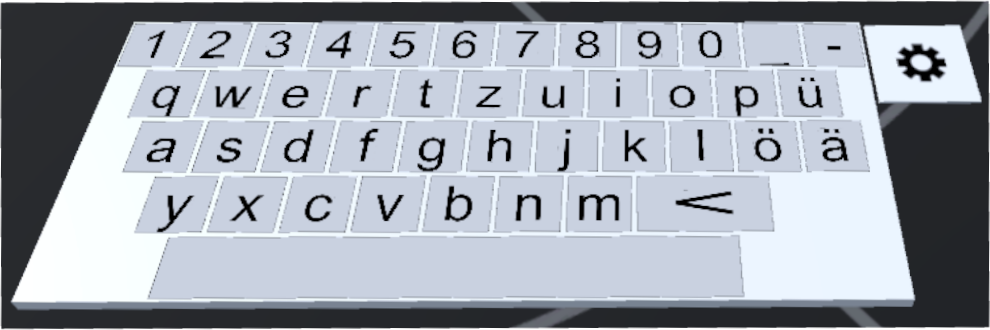
\includegraphics[width=0.7\textwidth]{WGKnormal}
\caption{Word-gesture keyboard in its ``normal'' form without anything selected}
%\label{fig:machine}
\end{figure}
    
\subsection{Text input}
There should be two text input methods for the user. One is the input of words with gestures, the other one is the input of single characters by tapping single keys.

\begin{figure}
\centering
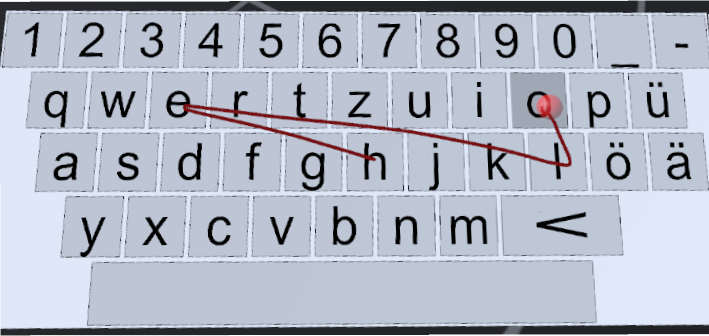
\includegraphics[width=0.4\textwidth]{WGKwrite}
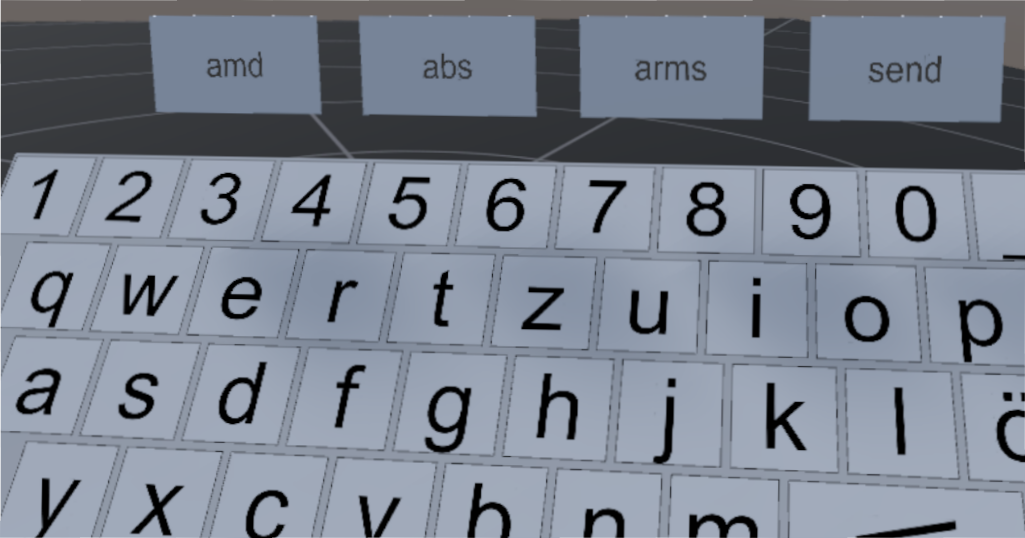
\includegraphics[width=0.4\textwidth]{WGKsuggestions}
\caption{left: the user writes the word ``hello'' as gesture, right: user gets recommended words for ``and''}
\label{fig:write_suggestions}
\end{figure}

\subsubsection{With Gestures}
The most important function our word-gesture keyboard provides, is the writing of words with gestures. A user can press and hold the trigger button of a VR controller inside the keyboard's hitbox and start making a gesture on it. The user will see a red line, that is drawn on the keyboard where they gesture. This helps them to keep track of the line they drew. When the user wants to finish the gesture, they need to release the trigger of the controller. At this moment, our program starts to evaluate the 5 words with the best match to the user inputted graph. The one with the highest confidence score will be written into the text field. The other 4 are displayed at the keyboard (fig \ref{fig:write_suggestions} right), such that the user can also choose between them. When they choose one of these 4 words, the word that has been written into the text field before, is replaced by the chosen word and the button, where the chosen word was written, will then display the replaced word.\\
There are some challenges in VR we have to master. First of all, in VR the user is in a three-dimensional space. Thus, when they make a gesture, they could move up and down with their controller and do not have to stay on the keyboard. For this we need to look, that the line of the gestures still lies on the keyboard as if the user would draw on it as if it was paper, and they are using a pen. The next problem is, that a user can rotate the keyboard as they want in VR. Therefore, the drawn graph will most of the time not be lieing perfectly on the x-z-plane. This means, we have to transform all the points into the x-z-plane to be able to further process these gestures. Another problem of the inputting of gestures is the amount of points. Technically seen, every frame the user presses draws a gesture, a new point gets saved. Thus, we have to reduce this amount, because it would be just too many points, and it would slow down the program massively. We implemented a function that only TODO: ÜBERPRÜFEN. keeps points of they have either a certain distance between itself and the previous point, or there is a big enough angle.

\subsubsection{As Single Characters}
If the wanted word is not in the lexicon, there will not be any entry in any layout file. Therefore, our algorithm will not be able to get this wanted word as best match, hence it can not be written as gesture. For this case, we need a method to input single characters. Fortunately with our word-gesture keyboard this almost works without additional work. If the single letters are in the layout files, the user is technically seen able to write single letters with a gesture. This ``gesture'' would just be a point on the right key, hence a single click at the right position. But there might be a little inconvenience. This is caused by the fact, that we work with distances. The distance from one letter to another is not big. And if for example the user wants to write an ``e'' but presses the key with the ``e'' on it on its left side and not perfectly in the middle, our system would also evaluate that aside from ``e'', also ``w'' and ``we'' are words, the user might have intended to write (on a conventional qwertz or qwerty layout). To avoid this, our system checks, if the user inputted graph's bounding box is smaller than TODO: HOW MUCH SMALLER?. It recognizes, that the user wants to write a single letter, and then takes the best match. To get back to the example, ``we'' would be discarded and ``e'' would get a higher score than ``w'', because of a smaller location channel distance. Therefore, the written ``word'' in this case would be ``e''.

\subsubsection{Spaces and Backspaces} TODO: WRITE IF KNOWN ABOUT THE VITRIVR FUNCTIONS
Important when writing more than one word or characters are spaces. When the user writes a word that consists of more than one character, a space gets put behind the word TODO: MIGHT CHANGE WITH IMPLEMENTATION. This means, if they write a second word, they do not have to put a space manually. But if they write a single character, no space is put automatically.\\
When the user writes a word and then uses the backspace key, the whole word gets deleted. After this first word, only single characters will be deleted afterwards.

\subsection{Create New Layouts}
Another function is the creation of custom layouts. While this would not be a necessary function to reach the core goal of inputting text, it can still help users to feel more confident using the keyboard. For example, if we only implement the qwertz layout, a user that is only using keyboards with the qwerty, ATOMIK or any other layout than qwerty, it can be cumbersome for them to use this keyboard. The problem is, that we do not know every layout all users are using for non-VR text input. Therefore, it is good that a user can decide by themselves what layout they like most to use and simply create it for our word-gesture keyboard.\\
TO achieve the creation of new layouts, a text file for layouts exists, that contains all available layouts. The user can create as many new layouts as they want to. To create a new one, the user has to write the new layout's name on the first new line. On the following lines they have to write the characters in an order, in which they want to have them on the keyboard. All the Unicode characters should be working, but two. In the current implementation, one whitespace is used to declare the position of the spacebar and the ``$<$'' character is used for the backspace key. This file gets read at the start of the program, so it cannot be edited while the program is running, or to be precise, the changes will not be recognized during runtime. One smaller thing we implemented is, that at the start of the program all characters used in the layouts not yet in the lexicon text file and layout files are being added. Without doing this, the user might not be able to input some single characters with their newly created keyboard, because the system simply would not find them in the layout files. During the runtime, the user then is able to switch between available layouts.

\subsection{Options}

\begin{figure}
    \centering
    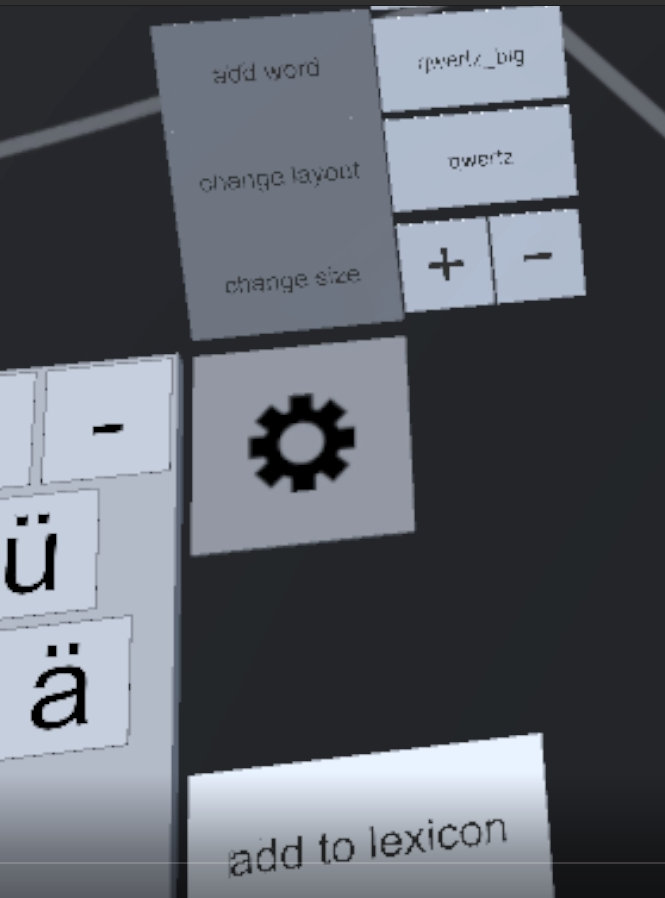
\includegraphics[width=0.4\textwidth]{WGKoptions}
    \caption{The options button with all the sub-buttons activated}
    \label{fig:options}
\end{figure}

To let the user use the other functions, we implemented an options button for our keyboard. It is marked with a black gear as seen in fig \ref{fig:options}. The user can click on it with the trigger button of the controller when being in the hitbox of it. Then, three new buttons appear, each for one currently available option. One is to add new words, one to change the currently selected layout and the last one to scale the keyboard.

\subsubsection{Add Words}
\begin{figure}
    \centering
    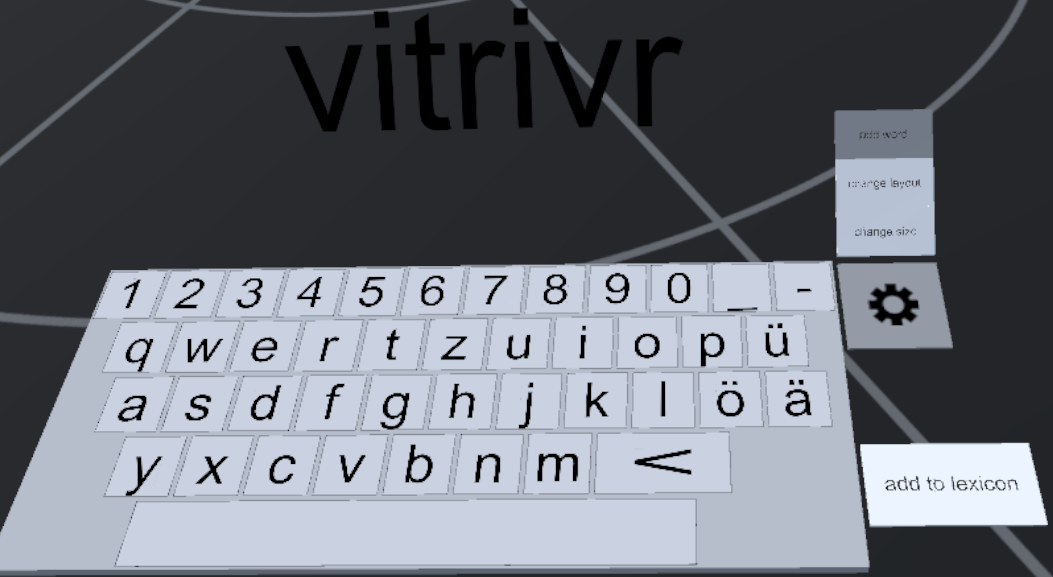
\includegraphics[width=0.4\textwidth]{WGKaddword}
    \caption{``vitrivr'' written with single character inputs, can now be added to the lexicon}
    \label{fig:addword}
    %\label{fig:machine}
\end{figure}
The whole system works with a lexicon full of words and only these can be written with gestures. There will be words the user wants to write, that are not yet in said lexicon, hence they can not be written with gestures. For this case, we implemented a function such that the user can add new words. They can access it via the options button. Then they have to press the button where it says ``add word''. When this button is pressed another button appears, the ``add to lexicon'' button. Now, the user has to input their intended word with single characters. It will be displayed as seen in Figure \ref{fig:addword}. Then, when they press the ``add to lexicon'' button, this displayed word will be added to the lexicon text file, if it does not already exist, and does not have a space in it. Additionally, for every available layout, the newly added word will also be added to the corresponding layout file, such that the user can, right after adding the word, write it with a gesture. One additional thing we implemented is, that the word only gets added in the text files, if it can be written with the layout the file corresponds to. For example, if a user wants to add the word ``öffentlich'', but they made a layout without the letter ``ö'', this word could never be written with this layout, hence it would be unnecessary to have it in the corresponding layout file.

\subsubsection{Change Scale and Layout}
There are two other functions that can be found under the options button. One is to change the size of the keyboard. When the user clicks on the ``change scale'' button, a ``+'' and a ``-'' button appear. By pressing the ``+'' button, the keyboard gets bigger, by pressing the ``-'' button, the keyboard gets smaller. This can help the user to make the keyboard more handy for them. Depending on how they want to move their arm, they can make it slightly bigger or smaller. If it is bigger, the gestures can be made more precise, if it is smaller, gestures can be made faster.\\
The other function is the ability to change the layout. The user gets a list of all available layouts, when pressing the ``change layout'' button. They can then click on one of these layouts and the keyboard will change its appearance. The available layouts consist of the predefined ones and also of the newly added ones from the user.

\subsection{Moving and Rotating}
Finally, we will briefly talk about the last function, the ability to grab and move the keyboard. This means, the user can grab the keyboard, by being in its hitbox and pressing and holding the controller's grip button. They can move it around in the room and rotate it as they want. If they release the grip button, the keyboard gets static and stays in the position.\\
This function can become handy, if the user wants to reposition themselves in the VR space. They can just take the keyboard with them. Also, they can choose to have it closer or futher away, which can lower the cumbersomeness to use the keyboard. Rotating the keyboard can also help this purpose. Some users might prefer to have it more tilted than other do.